\documentclass[11pt,letterpaper, leqno]{article}
\usepackage{latexsym}
\usepackage{amsmath}
\usepackage{amssymb}
\usepackage{amsthm}
\topmargin -0.25in
\textheight 8.5in
\oddsidemargin 0.0in
\textwidth 6.5in

\RequirePackage{amsthm,amsmath,amsfonts,amssymb}
%\RequirePackage[numbers]{natbib}
\RequirePackage[authoryear]{natbib}%% uncomment this for author-year citations
\RequirePackage[colorlinks,citecolor=blue,urlcolor=blue]{hyperref}%% uncomment this for coloring bibliography citations and linked URLs
\RequirePackage{graphicx}%% uncomment this for including figures

\usepackage{natbib}
\usepackage{authblk}
\usepackage[english]{babel}
\bibliographystyle{abbrvnat}
\setcitestyle{authoryear,open={(},close={)}}

% For the algorithm table
\usepackage{algorithm,algcompatible,amsmath}
\DeclareMathOperator*{\argmax}{\arg\!\max}
\DeclareMathOperator*{\argmin}{\arg\!\min}
% https://tex.stackexchange.com/q/83169/5764
\algnewcommand\INPUT{\item[\textbf{Input:}]}%
\algnewcommand\OUTPUT{\item[\textbf{Output:}]}%
%



\newtheorem{theorem}{Theorem}
\newtheorem{acknowledgement}[theorem]{Acknowledgement}
%\newtheorem{algorithm}[theorem]{Algorithm}
\newtheorem{axiom}[theorem]{Axiom}
\newtheorem{problem}[theorem]{Problem}
\newtheorem{remark}{Remark}
\newtheorem{claim}[theorem]{Claim}
\newtheorem{conclusion}[theorem]{Conclusion}
\newtheorem{condition}[theorem]{Condition}
\newtheorem{conjecture}[theorem]{Conjecture}
\newtheorem{corollary}{Corollary}
\newtheorem{criterion}[theorem]{Criterion}
\newtheorem{definition}{Definition}
\newtheorem{example}{Example}
\newtheorem{exercise}[theorem]{Exercise}
\newtheorem{lemma}{Lemma}
\newtheorem{proposition}{Proposition}
\newtheorem{thm}{Theorem}[section]
\newtheorem{lem}{Lemma}[section]
\newtheorem{prop}{Proposition}[section]
\newtheorem{defn}{Definition}[section]
\newtheorem{ex}{Example}[section]
\newtheorem{cor}{Corollary}[section]
\newtheorem{rem}{Remark}[section]
\newtheorem{rems}{Remarks}[section]
\numberwithin{equation}{section} 
\numberwithin{theorem}{section}
\numberwithin{lemma}{section} 
\numberwithin{corollary}{section}
\numberwithin{definition}{section}
\numberwithin{proposition}{section} 
\numberwithin{remark}{section}
\numberwithin{example}{section}
\newtheorem{assumption}{Assumption}
\DeclareMathOperator\supp{supp}

%\newcommand{\ex}{{\bf\sf E}}            %% expectation
\newcommand{\bfp}{{\bf P}}
\newcommand{\bfr}{{\bf R}}
\newcommand{\Var}{{\rm Var}}            %% 
\newcommand{\Cov}{{\rm Cov}}            %% 
\newcommand{\calc}{{\cal C}}            %%
\newcommand{\cald}{{\cal D}} 
\newcommand{\calf}{{\cal F}}            %%
\newcommand{\call}{{\cal L}}            
\newcommand{\al}{\alpha}                %%
\newcommand{\bt}{\beta}                %%
\newcommand{\ga}{\gamma}                %% abbreviated
\newcommand{\dt}{\delta}                %% greek letters
\newcommand{\la}{\lambda}               %%
\newcommand{\ep}{\epsilon}              %%
\newcommand{\sig}{\sigma}               %%
\newcommand{\tri}{\triangle}
\newcommand{\om}{\omega}                %%
\newcommand{\ra}{\rightarrow}           %%
\newcommand{\lra}{\longrightarrow}
\newcommand{\Ra}{\Rightarrow}           %% arrows
\newcommand{\subs}{\subseteq}           %% subset or equal to
\newcommand{\eqdef}{\stackrel{\triangle}{=}}
\newcommand{\hY}{\hat{Y}}
\newcommand{\hp}{\hat{p}}
\newcommand{\hX}{\hat{X}}
\newcommand{\hy}{\hat{y}}
\newcommand{\hQ}{\hat{Q}}
\newcommand{\Zh}{\hat{Z}}
\newcommand{\hla}{\hat{\lambda}}
\newcommand{\starti}{\parindent0pt\it}  %% start an italic line
\newcommand{\startb}{\parindent0pt\bf}  %% start a boldface line
\newcommand{\tril}{\triangle^-}
\newcommand{\trir}{\triangle^+}
\newcommand{\trilr}{\triangle^{\pm}}
\newcommand{\realR}{{{\rm I}\;\!\!\!{\rm R}}}
\newcommand{\probP}{{{\rm I}\;\!\!\!{\rm P}}}
\newcommand{\filtF}{{{\rm I}\;\!\!\!{\rm F}}}
\newcommand{\expeE}{{{\rm I}\;\!\!\!{\rm E}}}
\newcommand{\noin}{{\noindent}}
\newcommand{\doty}{{\dot{y}}}
\newcommand{\doth}{{\dot{h}}}
\newcommand{\dotx}{{\dot{x}}}
\newcommand{\dotu}{{\dot{u}}}
\newcommand{\dotf}{{\dot{f}}}
\newcommand{\dotg}{{\dot{g}}}
\newcommand{\ddoty}{{\ddot{y}}}
\newcommand{\ddoth}{{\ddot{h}}}
\newcommand{\ddotx}{{\ddot{x}}}
\newcommand{\ddotf}{{\ddot{f}}}
%\newcommand{\Var}{{\mbox{Var}}}
%\newcommand{\Cov}{{\mbox{Cov}}}
\newcommand{\T}{\intercal}

\newcommand{\ans}[1]{\boxed{\text{#1}}}
\newcommand{\vecs}[1]{\langle #1\rangle}
\renewcommand{\hat}[1]{\widehat{#1}}
\newcommand{\F}[1]{\mathcal{F}(#1)}
\renewcommand{\P}{\mathbb{P}}
\newcommand{\R}{\mathbb{R}}
\newcommand{\E}{\mathbb{E}}
\newcommand{\Z}{\mathbb{Z}}
\newcommand{\ind}{\mathbbm{1}}
\renewcommand{\qed}{\quad \blacksquare}
\newcommand{\brak}[1]{\left\langle #1 \right\rangle}
\newcommand{\bra}[1]{\left\langle #1 \right\vert}
\newcommand{\ket}[1]{\left\vert #1 \right\rangle}
\newcommand{\mfX}{\mathfrak{X}}

\begin{document}
\begin{center}
{\bf \Large APMA1690: ~~Homework \# 7 ~~~(Due by 11pm on November 9)}
\end{center}
\[\]
\medskip

\section{Review}

I would suggest you go through the review section before going to the problem set.

%\subsection{Notations}
%\begin{itemize}
%    \item a
%\end{itemize}

\subsection{Markov Chains vs. Markov Chain Monte Carlo}

When we were talking about (homogeneous\footnote{All the Markov chains referred to in APMA 1690 are homogeneous Markov chains.}) Markov chains, we were in a situation where a transition probability $p(x,y)$ of a Markov chain was given; we were asked to derive a/the stationary distribution $\pi$ associated with $p(x,y)$.

We are now learning the theory of Markov Chain Monte Carlo (MCMC), and the situation is reversed --- a distribution $\pi$ is given, and we are asked to derive a transition probability $p(x,y)$ satisfying the following requirements
\begin{itemize}
    \item the Markov chain associated with $p(x,y)$ is irreducible and aperiodic;
    \item the given distribution $\pi$ is the stationary distribution of the Markov chain. (Since the Markov chain is irreducible, we are safe to use the phrase ``\textbf{the} stationary distribution.")
\end{itemize}

\subsection{Asymptotic Behaviors of Markov Chains}

The MCMC method needs some asymptotic results about Markov chains as its theoretical foundations.

\begin{theorem}\label{thm: asymptotic distributions of MCs}
Let $\{X_n\}_{n=0}^\infty$ be a homogeneous Markov chain taking values in a finite state space $\mathcal{X}=\{x_1,\ldots,x_S\}$. If this Markov chain is \textbf{irreducible} and \textbf{aperiodic}, we have 
\begin{align}\label{eq: asymptotic distributions of Markov chains}
    \begin{aligned}
    & \lim_{n\rightarrow\infty}\mathbb{P}(X_n=x_j \,\vert\, X_0=x_i)=\pi(x_j),\ \ \mbox{equivalently} \\
    & \lim_{n\rightarrow\infty} (\boldsymbol{P}^n)_{ij}=\pi(x_j),\ \ \mbox{ for all }i,j\in\{1,2,\ldots,S\},
    \end{aligned}
\end{align}
where $\pi$ is the unique stationary distribution of the Markov chain.
\end{theorem}
\noindent Theorem \ref{eq: asymptotic distributions of Markov chains} further implies the following
\begin{align*}
    \lim_{n\rightarrow\infty}\mathbb{P}(X_n=x_j) 
    & =\sum_{i=1}^S \left[\lim_{n\rightarrow\infty}\mathbb{P}(X_n=x_j \,\vert\, X_0=x_i)\right]\cdot \mathbb{P}(X_0=x_i) \\
    & = \pi(x_j) \cdot \sum_{i=1}^S \mathbb{P}(X_0=x_i) \\
    & = \pi(x_j),\ \ \mbox{ for all }j=1,\ldots,S,
\end{align*}
that is, $X_n$ looks like a $\pi$-distributed random variable when $n$ is sufficiently large.

\subsection{Generating a Markov Chain from a Transition Probability}

For any transition probability function $p(x,y)$, when $x$ is fixed, the function $y\mapsto p(x,y)$ of $y$ is a PMF.

Suppose what we know is a transition probability function $p$, instead of a Markov chain. With $p$, using the following conceptual algorithm, we can generate a Markov chain whose transition probability is the given $p$.
\begin{algorithm}
\caption{: Generating Markov Chains}\label{algorithm: generating MCs with knowing how to deal with transition probability}
\begin{algorithmic}[1]
    \INPUT (i) transition probability $p$, and (ii) initialization $x_0$.
    \OUTPUT a Markov chain $\{X_n\}_{n=0}^\infty$ whose transition probability is $p$.
    \STATE $X_0\leftarrow x_0$.
    \FORALL{$n=1,2,\ldots$}
    \STATE Generate $X_{n}$ from the PMF $p(X_{n-1},\cdot)$.
    \ENDFOR
\end{algorithmic}
\end{algorithm}

\subsection{Main Theme of MCMC}

In many applications, the distribution $\pi$ of interest is defined in an extremely high-dimensional space. For example, if $\pi$ is the random 256-by-256 binary-valued pictures (i.e., each picture has $256\times 256$ pixels, and each pixel takes its value in the binary set $\{-1,1\}$), the $\pi$ is a PMF defined on a state space containing $2^{65536}$ elements.\footnote{Recall that $2^{10}=1023\approx 10^3$.} It is \textbf{infeasible} to generate random variables \textbf{exactly} following such a high-dimensional distribution.

Suppose we can generate a Markov chain $\{X_n\}_{n=0}^\infty$ satisfying the following requirements
\begin{itemize}
    \item $\{X_n\}_{n=0}^\infty$ is irreducible and aperiodic;
    \item the given distribution $\pi$ is the stationary distribution of $\{X_n\}_{n=0}^\infty$.
\end{itemize}
Then, we have the following
\begin{align*}
    \lim_{n\rightarrow\infty}\mathbb{P}(X_n=x)=\pi(x),\ \ \mbox{for all }x.
\end{align*}
Hence, when $n$ is large, $X_n$ \textbf{approximately} follows the given distribution $\pi$; we may approximately view $X_n$ as a random variable generated from $\pi$.

For a given distribution $\pi$, two widely adopted methods of generating such a Markov chain are ``Metropolis-Hastings algorithm" and ``Gibbs sampling."

\subsection{Metropolis-Hastings Algorithm}

\cite{metropolis1949monte} and \cite{metropolis1953equation} were the first to describe Markov chain simulation of probability distributions. The method is concluded as the ``Metropolis algorithm." \cite{hastings1970monte} generalized this algorithm.

Suppose $\pi$ is the distribution of interest, and it is strictly positive, i.e., 
\begin{align*}
    \pi(x)>0,\ \ \mbox{ for all }x\in\mathcal{X}.
\end{align*}

\subsubsection{Metropolis Algorithm}

Suppose we have a transition probability function $q(x,y)$ in hand, and $q(x,y)$ satisfies the following conditions
\begin{itemize}
    \item we know how to generate a Markov chain from $q(x,y)$ in an efficient way;
    \item $q(x,y)$ is symmetric, i.e., $q(x,y)=q(y,x)$ for all $x,y\in\mathcal{X}$.
\end{itemize}
The Metropolis algorithm generates a Markov chain with the following transition probability\footnote{The logic of Eq.~\eqref{eq: transition prob of the Metropolis algorithm} is the following: we first define $p(x,y)$ for all $x\ne y$, then we define $p(x,x)=1-\sum_{z:z\ne x} p(x,z)$.}\footnote{You may ask, \textit{why is $p(x,x)$ defined separately?} Answer: If we simply define $p(x,x)=q(x,x)$, then $p$ would not be a transition probability. The transition probability assumption requires $1=\sum_{y\in\mathcal{X}} p(x,y)$. However, $\frac{\pi(y')}{\pi(x)}$ can be strictly smaller than 1 for some $y'\ne x$. In this scenario, if we did not define $p(x,x)$ separately --- that is, we define $p(x,x)=q(x,x)$, we will have 
\begin{align*}
    1=\sum_{y\in\mathcal{X}}p(x,y)=\sum_{y\in\mathcal{X}} q(x,y)\cdot \min\left\{1, \, \frac{\pi(y)}{\pi(x)}\right\}=q(x,x)+\sum_{y\ne x,y'} q(x,y)\cdot \min\left\{1, \, \frac{\pi(y)}{\pi(x)}\right\} + q(x,y')\cdot \min\left\{1, \, \frac{\pi(y')}{\pi(x)}\right\}<\sum_{y\in\mathcal{X}}q(x,y)=1,
\end{align*}
which is a contradiction. Hence, we need to define $p(x,x)$ separately to correct for the ``loss of mass" in the term $q(x,y')\cdot \min\left\{1, \, \frac{\pi(y')}{\pi(x)}\right\}$.
}
\begin{align}\label{eq: transition prob of the Metropolis algorithm}
    p(x,y) = \left\{
    \begin{aligned}
    & q(x,y)\cdot\min\left\{1, \, \frac{\pi(y)}{\pi(x)}\right\},\ \ &&\mbox{ if }x\ne y, \\
    & 1-\sum_{z:z\ne x} p(x,z),\ \ &&\mbox{ if }x=y,
    \end{aligned}
    \right.
\end{align}
for all $x,y\in\mathcal{X}$, where ``$\sum_{z:z\ne x}$" denotes the sum across all $z\in\mathcal{X}$ that are not equal to $x$.

The following claims show that the $p(x,y)$ defined in Eq.~\eqref{eq: transition prob of the Metropolis algorithm} works.
\begin{claim}\label{claim 1}
If $q(x,y)$ is irreducible and aperiodic\footnote{It actually means, ``the Markov chain associated with $q(x,y)$ is irreducible and aperiodic;" for $p(x,y)$, similarly.}, then $p(x,y)$ is irreducible and aperiodic.
\end{claim}

\emph{Proof:} See the problem set section.

\begin{claim}\label{claim 2}
The $p(x,y)$ defined by Eq.~\eqref{eq: transition prob of the Metropolis algorithm} satisfies the following equation\footnote{If $\pi$ satisfies Eq.~\eqref{eq: reversible reversible distribution}, it is called a \href{https://inst.eecs.berkeley.edu/~ee126/sp18/reversibility.pdf}{reversible distribution} of the transition probability $p$ (see Example 6.5.4 of \cite{durrett2019probability} or Eq. (18.8) of \cite{klenke2013probability}).}
\begin{align}\label{eq: reversible reversible distribution}
    \pi(x)p(x,y)=\pi(y)p(y,x),\ \ \mbox{ for all }x,y\in\mathcal{X}.
\end{align}
\end{claim}

\emph{Proof:} See the problem set section.

\begin{claim}\label{claim 3}
$\pi$ is a stationary distribution of $p$.
\end{claim}

\emph{Proof:} It comes from Claim \ref{claim 2}. Specifically, Eq.~\eqref{eq: reversible reversible distribution} implies
    \begin{align*}
        \sum_{y\in\mathcal{X}}\pi(x)p(x,y)=\sum_{y\in\mathcal{X}}\pi(y)p(y,x),
    \end{align*}
    where the left-hand side is equal to $\pi(x) \sum_{y\in\mathcal{X}} p(x,y)=\pi(x)$. Therefore, $\pi(x) = \sum_{y\in\mathcal{X}}\pi(y)p(y,x)$.

Algorithm \ref{algorithm: Metropolis algorithm} can generate a Markov chain whose transition probability is the $p(x,y)$ defined in Eq.~\eqref{eq: transition prob of the Metropolis algorithm}.
\begin{algorithm}
\caption{: Metropolis Algorithm}\label{algorithm: Metropolis algorithm}
\begin{algorithmic}[1]
    \INPUT (i) the distribution $\pi$ of interest satisfying $\pi(x)>0$ for all $x\in\mathcal{X}$; (ii) a jumping distribution --- a symmetric transition probability $q$ of an irreducible and aperiodic Markov chain; (iii) an initial starting point $x_0$; (iv) a large integer $n^*$.
    \OUTPUT The first $n^*$ components of a Markov chain $\{X_n\}_{n=0}^\infty$ with $\pi$ as its stationary distribution.
    \STATE Initialize $X_0 \leftarrow x_0$.
    \FORALL{$n=1, 2,\ldots, n^*$}
    \STATE Sample a proposal $X^*$ from the PMF $q(X_{n-1},\, \cdot\,)$.
    \STATE Compute the ratio $r\leftarrow\frac{\pi(X^*)}{\pi(X_{n-1})}$. (Remark: Since we assume that $\pi(x)>0$ for all $x\in\mathcal{X}$, the ratio $r$ is always well-defined.)
    \STATE Generate $Y\sim \operatorname{Bernoulli}(\min\{r,1\})$, i.e., $\mathbb{P}(Y=1)=\min\{r,1\}$.
    \STATE $X_n \leftarrow Y\cdot X^* + (1-Y)\cdot X_{n-1}$.
    \ENDFOR
\end{algorithmic}
\end{algorithm}

\subsubsection{Metropolis-Hastings Algorithm}

The Metropolis algorithm requires $q(x,y)$ to be symmetric. This symmetry condition can be removed by modifying Eq.~\eqref{eq: transition prob of the Metropolis algorithm} to the following form, which results in the Metropolis-Hastings algorithm.
\begin{align}\label{eq: Metropolis-Hastings matrix}
    p(x,y):=\left\{
    \begin{aligned}
    & q(x,y)\cdot\min\left\{1, \frac{\pi(y)\cdot q(y,x)}{\pi(x)\cdot q(x,y)}\right\},\ \ &&\mbox{ if }x\ne y \mbox{ and }q(x,y)>0, \\
    & 0, \ \ &&\mbox{ if }x\ne y \mbox{ and }q(x,y)=0, \\
    & 1-\sum_{z:z\ne x} p(x,z), \ \ &&\mbox{ if }x=y,
    \end{aligned}
    \right.
\end{align}
for all $x,y\in\mathcal{X}$, where ``$\sum_{z:z\ne x}$" denotes the sum across all $z$'s that are not equal to $x$. The only difference between Eq.~\eqref{eq: transition prob of the Metropolis algorithm} and Eq.~\eqref{eq: Metropolis-Hastings matrix} is that the $q(x,y)$ in Eq.~\eqref{eq: Metropolis-Hastings matrix} is no longer required to be symmetric.

The following theorem is Theorem 18.15 of \cite{klenke2013probability} and provides the theoretical foundation for the Metropolis-Hastings algorithm
\begin{theorem}\label{thm: Theorem 18.15 of Klenke}
Assume that $q$ is irreducible and that for any $x,y\in\mathcal{X}$, we have $q(x,y)>0$ if and only if $q(y,x)>0$. Then the transition probability $p$ defined in Eq.~\eqref{eq: Metropolis-Hastings matrix} is irreducible and has the unique stationary distribution $\pi$. If, in additon, $q$ is aperiodic, then $p$ is aperiodic as well.
\end{theorem}

Algorithm \ref{algorithm: Metropolis-Hastings algorithm} can generate a Markov chain whose transition probability is the $p(x,y)$ defined in Eq.~\eqref{eq: Metropolis-Hastings matrix}.
\begin{algorithm}
\caption{: Metropolois-Hastings Algorithm}\label{algorithm: Metropolis-Hastings algorithm}
\begin{algorithmic}[1]
    \INPUT (i) the distribution $\pi$ of interest; (ii) a jumping distribution --- a transition probability $q$ of an irreducible and aperiodic Markov chain; (iii) an initial starting point $x_0$.
    \OUTPUT A Markov chain $\{X_n\}_{n=0}^\infty$ with $\pi$ as its stationary distribution.
    \STATE Set $X_0 \leftarrow x_0$.
    \FORALL{$n=1,2,\ldots$}
    \STATE Sample a proposal $X^*$ from the PMF $q(X_{n-1},\, \cdot)$.
    \STATE Compute the ratio $r\leftarrow\frac{\pi(X^*)\cdot q(X^*, X_{n-1})}{\pi(X_{n-1})\cdot q(X_{n-1}, X^*)}$. (Remark: If $q(X_{n-1}, X^*)=0$, then it is almost impossible to sample $X^*$ in the preceding step. So, the ratio $r$ is well-defined with probability one.)
    \STATE Generate $Y\sim \operatorname{Bernoulli}(\min\{r,1\})$.
    \STATE $X_n \leftarrow Y\cdot X^* + (1-Y)\cdot X_{n-1}$.
    \ENDFOR
\end{algorithmic}
\end{algorithm}


\subsection{Applications of MCMC}

When you were learning the theoretical foundation of MCMC (i.e., Theorem \ref{thm: asymptotic distributions of MCs}), you assumed that state spaces are finite. In applications, people directly use these MCMC formulas/algorithms for general scenarios, e.g., state spaces are infinite and continuous. It usually works because of the following
\begin{itemize}
    \item The theoretical foundation for the general scenarios exists, although it involves very advanced mathematical tools and requires more conditions (e.g., see \cite{tierney1994markov} and \cite{athreya1996convergence}).
    \item In computers, everything is discrete and finite.
\end{itemize}
We will also adopt the application convention and apply the Metropolis-Hastings algorithm/Gibbs sampling to general scenarios, e.g., continuous distributions defined on continuous state spaces.


\newpage

\section{Problem Set}

\begin{enumerate}

\item (3 points) Suppose $q(x,y)$ is the transition probability of a Markov chain, and $q(x,y)$ is symmetric, i.e., $q(x,y)=q(y,x)$ for all $x,y\in\mathcal{X}$. Let $p(x,y)$ be the function defined by Eq.~\eqref{eq: transition prob of the Metropolis algorithm}. \textbf{Prove Claim \ref{claim 1}.}

    \color{blue}
        \textbf{Claim:} If $q(x, y)$ is irreducible and aperiodic, then $p(x, y)$ is irreducible and aperiodic. 

        Because $q(x, y) = q(y, x) \qquad \forall x, y \in \mfX$, it is clear that if $q(x, y) > 0$, then $q(y, x) > 0$ and vice versa. Then since $q$ is irreducible and aperiodic, then by Theorem 1.5, the MC generated from 
        \begin{align*}
            p(x,y)=\left\{
                \begin{aligned}
                & q(x,y)\cdot\min\left\{1, \frac{\pi(y)\cdot q(y,x)}{\pi(x)\cdot q(x,y)}\right\},\ \ &&\mbox{ if }x\ne y \mbox{ and }q(x,y)>0, \\
                & 0, \ \ &&\mbox{ if }x\ne y \mbox{ and }q(x,y)=0, \\
                & 1-\sum_{z:z\ne x} p(x,z), \ \ &&\mbox{ if }x=y,
                \end{aligned}
                \right.
        \end{align*}
        is also irreducible and aperiodic. 

        However, this formula can be simplified. By the symmetry of $q$, 
        \[\min\{1, \frac{\pi(y)q(y, x)}{\pi(x)q(x, y)}\} = \min\{1, \frac{\pi(y)}{\pi(x)}\}\]
        In this version, if $q(x, y) = q(y,x) = 0$, there is no risk of division by $0$ so we can combine the cases $q =0$ and $q > 0$. Thus, we have that the MC generated by 
        \[p(x, y) = \begin{cases}
            q(x, y)\cdot \min \{1, \frac{\pi(y)}{\pi(x)}\}\qquad q(x, y) \geq 0\\
            1 - \sum_{z:z\neq x} p(x, z) \hspace*{2in} x = y
        \end{cases}\]
        is irreducible and aperiodic, which is exactly what we were trying to prove! $\qed$
    \color{black}

\pagebreak

\item (3 points) Suppose $q(x,y)$ is the transition probability of a Markov chain, and $q(x,y)$ is symmetric, i.e., $q(x,y)=q(y,x)$ for all $x,y\in\mathcal{X}$. Let $p(x,y)$ be the function defined by Eq.~\eqref{eq: transition prob of the Metropolis algorithm}. \textbf{Prove Claim \ref{claim 2}.}

    \color{blue}
        \textbf{Claim:} $\pi(x)p(x, y) = \pi(y) p(y, x) \qquad \forall x, y\in \mfX$ with 
        \[p(x,y) = \left\{
            \begin{aligned}
                & q(x,y)\cdot\min\left\{1, \, \frac{\pi(y)}{\pi(x)}\right\},\ \ &&\mbox{ if }x\ne y, \\
                & 1-\sum_{z:z\ne x} p(x,z),\ \ &&\mbox{ if }x=y,
            \end{aligned}
            \right.\]

        \emph{Proof:}
        
        If $y = x$, then clearly 
        \[\pi(x)p(x, y) = \pi(y) p(y, x)\]
        and we are done. 

        Otherwise, 
        \begin{align*}
            \pi(x)p(x, y) &= \pi(x) q(x,y)\cdot\min\left\{1, \, \frac{\pi(y)}{\pi(x)}\right\}\\
        \end{align*}

        This gives us two more cases.

        If $\pi(x) > \pi(y)$, then $\min\left\{1, \, \frac{\pi(y)}{\pi(x)}\right\} = \frac{\pi(y)}{\pi(x)}$, so
        \begin{align*}
            \pi(x)p(x, y) &= \pi(x)q(x, y)\cdot \frac{\pi(y)}{\pi(x)}\\
            &= \pi(y)q(x, y)\\
            &= \pi(y)q(y, x)
        \end{align*}
        Since $q(y, x) = \frac{p(y, x)}{\min\{1, \frac{\pi(x)}{\pi(y)}\}}$
        and $\pi(x) > \pi(y)$, the denominator is $1$ and $q(y, x) = p(y, x)$ so
        \[\pi(x)p(x, y) = \pi(y)p(y, x)\]

        Finally, if $\pi(x) \leq \pi(y)$, then $\min\left\{1, \, \frac{\pi(y)}{\pi(x)}\right\} = 1$, so 
        \[\pi(x)p(x, y) = \pi(x)q(x, y) = \pi(x)q(y, x)\]

        As above, 
        \[q(y, x) = \frac{p(y, x)}{\min\{1, \frac{\pi(x)}{\pi(y)}\}}\]
        but the min function equals $\frac{\pi(x)}{\pi(y)}$ so 
        \[q(y, x) = \frac{\pi(y)}{\pi(x)} p(y, x)\]
        and 
        \[\pi(x)q(y, x) = \pi(y)p(y,x)\]
        So 
        \[\pi(x)p(x, y) = \pi(y)p(y, x)\]
        for all $x, y \in \mfX. \qed$
    \color{black}

\pagebreak

\item (An application of the Metropolis algorithm) The distribution $\pi$ of interest is the PDF of the following \href{https://en.wikipedia.org/wiki/Multivariate_normal_distribution}{multivariate normal distribution}
\begin{align*}
    N\left(\begin{pmatrix}
        0 \\
        0
    \end{pmatrix}, \begin{pmatrix}
        1 & 0.8 \\
        0.8 & 1
    \end{pmatrix}\right).
\end{align*}
The transition probability $q$ (see Eq.\eqref{eq: transition prob of the Metropolis algorithm}) is defined by the following: for each fixed $\boldsymbol{x}=(x_1,x_2)$, let $q(\boldsymbol{x},\,\cdot)$ be the PDF of the following multivariate normal distribution
\begin{align*}
    N\left(\begin{pmatrix}
        x_1 \\
        x_2
    \end{pmatrix}, \begin{pmatrix}
        \sigma^2 & 0 \\
        0 & \sigma^2
    \end{pmatrix}\right).
\end{align*}

    \color{blue}
        This code contains my implementation of the Metropolis algorithm and will be used in every part below:

        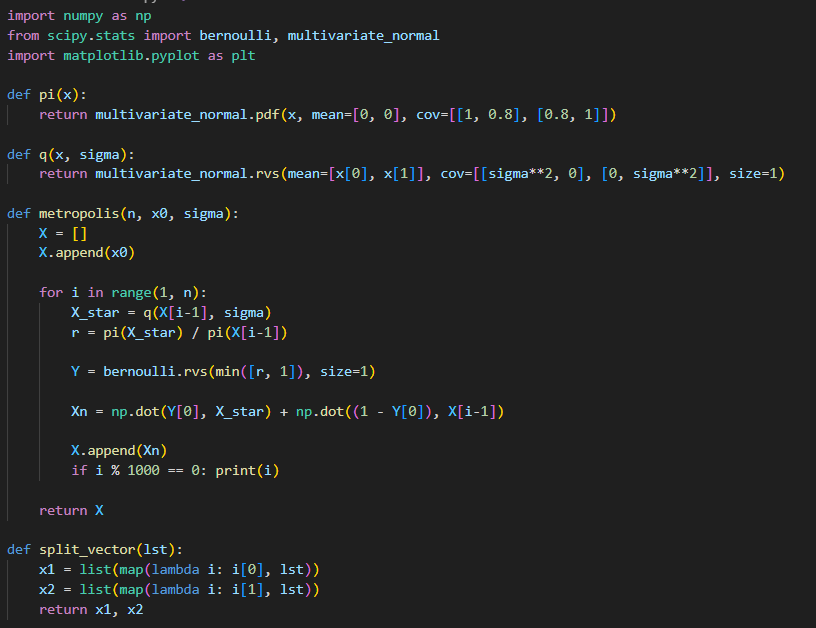
\includegraphics{Images/2. Code.png}

    \color{black}

\pagebreak
\begin{enumerate}
    \item (1 point) Let $\sigma=0.7$. Using $\pi$, $q$, and $\boldsymbol{x}_0=(-2,2)$ as inputs, generate the first 20,000 components of a Markov chain, i.e., $\{X_n\}_{n=0}^{20000}$, using the Metropolis algorithm (Algorithm \ref{algorithm: Metropolis algorithm}). Plot the second half of the sequence, i.e., $\{X_n\}_{n=10001}^{20000}$. Provide your code generating the plot. (Please feel free to use any code I uploaded to Canvas.)
    \item (0.5 points) Replace $\boldsymbol{x}_0$ with $(2,2)$ and repeat part (a).
    \item (0.5 points) Generate 20,000 data points from $\pi$ and plot these points. Provide your code generating the plot. 
    
    \color{blue}
        I generated the plots for A, B, and C together using this code:

        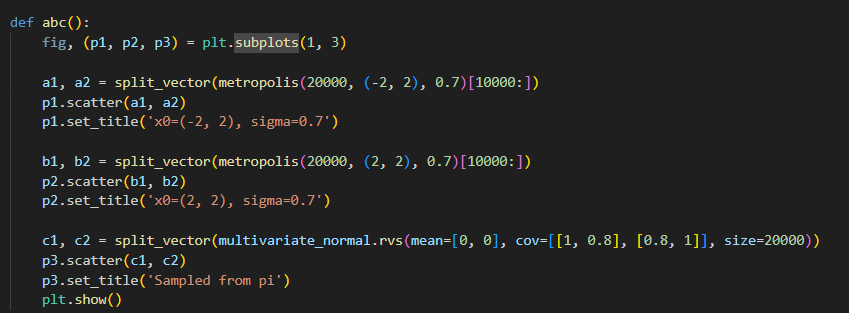
\includegraphics[width=\textwidth]{Images/2. ABC Code.png}

        which resulted in the following plot where the graph from part A is the lefmost subplot, part B is the center, and part C is the rightmost:

        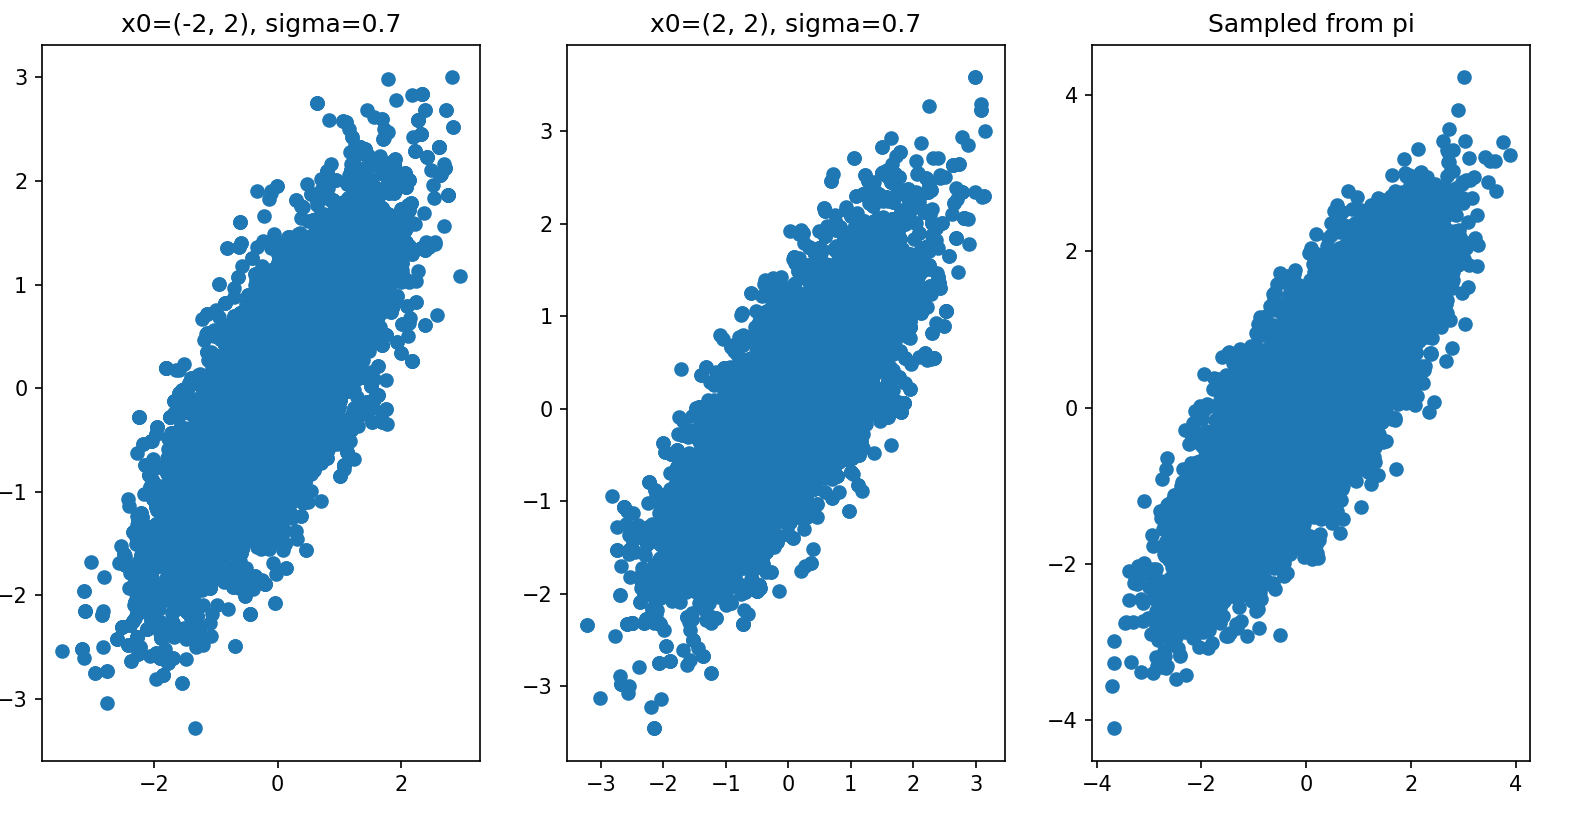
\includegraphics[width=\textwidth]{Images/2. ABC.png}
    \color{black}

    \pagebreak   
    \item (1 point) Replace $\sigma$ with $0.07$ and repeat part (a). Compare the plot you got in part (d) with the one you got in part (c). Are the two plots similar? If not, please explain the reason why they are not similar.
    
        \color{blue}
            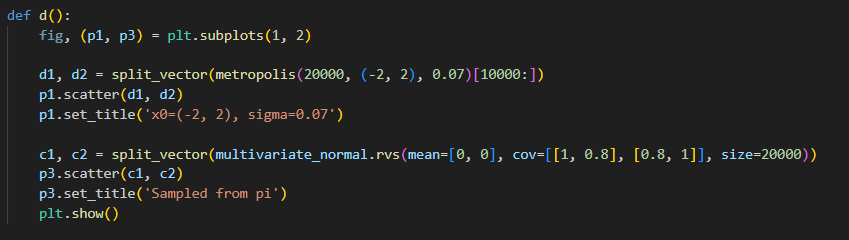
\includegraphics[width=\textwidth]{Images/2. D code.png}
            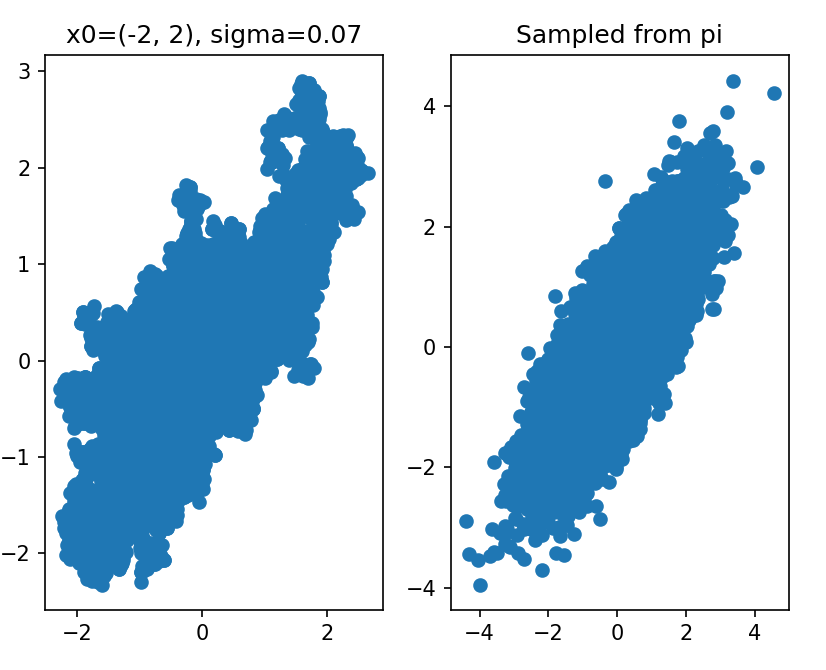
\includegraphics{Images/2. D.png}

            At first glance, the two plots look somewhat similar. On closer inspection, the plot limits do not align: the approximation in the left subplot ranges from $[-2, 2]$ in one dimension and $[-2, 3]$ in the other while the RVs sampled from $\pi$ are in the range $x_1 \in [-4, 4], x_2 \in [-4, 4]$. With very small $\sigma$, the distance between any $X^*$ and $X_{n-1}$ is small so $r = \frac{\pi(X^*)}{\pi(X_{n-1})}$ tends to $1$ so $Y \sim \text{Bernoulli}(\min\{1, 1\}) \to 1$ So $X_n \approx X^*$ and there is little change in the algorithm so it does not approximate $\pi$ very well. 
        \color{black}

    \pagebreak
    \item (1 point) Replace $\sigma$ with $70$ and repeat part (a). Compare the plot you got in part (e) with the one you got in part (c). Are the two plots similar? If not, please explain the reason why they are not similar.
    
        \color{blue}
            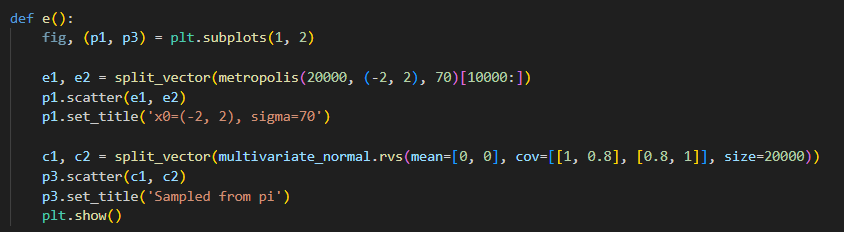
\includegraphics[width=\textwidth]{Images/2. E code.png}
            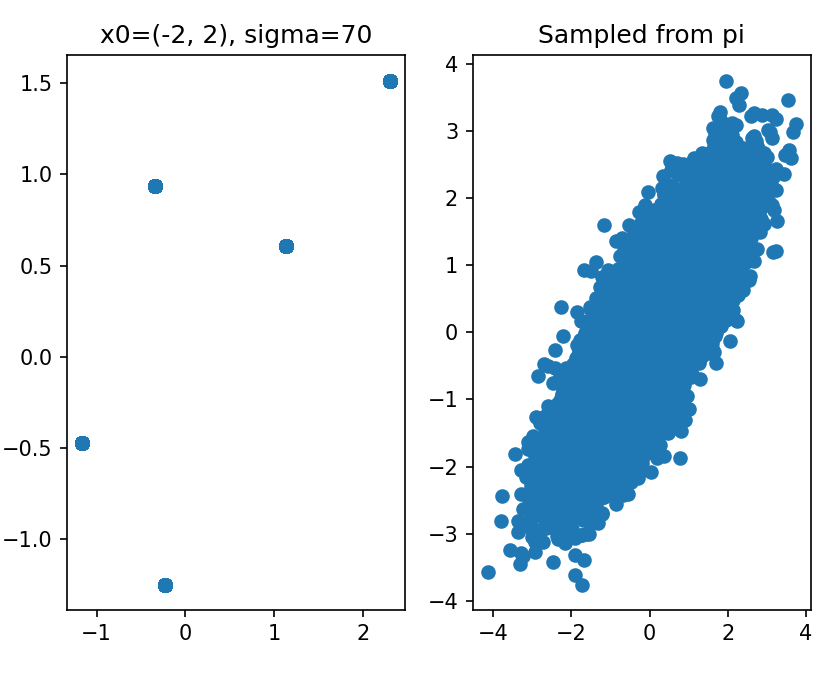
\includegraphics{Images/2. E.png}

            Like the above graph, this one does not resemble the plot of RVs drawn from $\pi$. When $\sigma$ is very large, $r = \frac{\pi(X^*)}{\pi(X_{n-1})}$ tends to be small so $Y$ tends to $0$ and $X_n \approx X_{n-1}$. As a result, the model ``gets stuck'' and only a few points are fit very often.
        \color{black}
\end{enumerate}

For either part (d) or part (e), try your best to make your explanations convincing to the TAs who grade this question.

Hints for parts (d) and (e): You may need to consider the following quantities
\begin{itemize}
    \item the distance between any two consecutive steps $X_{n-1}$ and $X_n$,
    \item the value $r  = \frac{\pi(X^*)}{\pi(X_{n-1})}$ in Algorithm \ref{algorithm: Metropolis algorithm} and the mechanism of $Y\sim \operatorname{Bernoulli}(\min\{1,r\})$.
\end{itemize}


\end{enumerate}


%\bibliographystyle{plain}
\bibliography{sample}

\end{document}
